\documentclass[numberedappendix]{emulateapj}
%\documentclass[iop]{emulateapj}
%apj gives the referee version/preprint2
%\usepackage[T1]{fontenc}
%\usepackage[utf8]{inputenc}
%\usepackage{graphicx}
%\usepackage{natbib}
\usepackage{amsmath}
\usepackage{amssymb}
%\usepackage{vmargin}
%\usepackage{pdfpages}
\usepackage{aas_macros}
\usepackage[normalem]{ulem}
\usepackage[usenames]{color}
\usepackage{bm}
\usepackage{cancel}
\definecolor{DarkGreen}{rgb}{0.64,0.80,0.35}
\newcommand\ALc[1]{{\color{red} \bf #1}} %Astrid
\newcommand\Ac[1]{{\color{green} \bf #1}} %% Avery
\newcommand\Pc[1]{{\color{cyan} \bf #1}} %% Phil
\newcommand\Cc[1]{{\color{blue} \bf #1}} %% Christoph
\newcommand\Ec[1]{{\color{magenta} \bf #1}} %% Ewald

\DeclareMathAlphabet\mathbfcal{OMS}{cmsy}{b}{n}
\newcommand{\calR}{\ensuremath{\bm\hat{\mathbfcal{R}}}}
\newcommand{\magcalR}{\ensuremath{\hat{\mathcal{R}}}}

\SetSymbolFont{symbols}{bold}{OMS}{cmsy}{b}{n}
%
\DeclareSymbolFont{bmisymbols}{OML}{cmm}{b}{it}
\DeclareMathSymbol{\balpha}{0}{bmisymbols}{"0B}
\DeclareMathSymbol{\bbeta}{0}{bmisymbols}{"0C}
\DeclareMathSymbol{\bgamma}{0}{bmisymbols}{"0D}
\DeclareMathSymbol{\bdelta}{0}{bmisymbols}{"0E}
\DeclareMathSymbol{\bepsilon}{0}{bmisymbols}{"0F}
\DeclareMathSymbol{\bzeta}{0}{bmisymbols}{"10}
\DeclareMathSymbol{\boldeta}{0}{bmisymbols}{"11}
\DeclareMathSymbol{\btheta}{0}{bmisymbols}{"12}
\DeclareMathSymbol{\biota}{0}{bmisymbols}{"13}
\DeclareMathSymbol{\bkappa}{0}{bmisymbols}{"14}
\DeclareMathSymbol{\blambda}{0}{bmisymbols}{"15}
\DeclareMathSymbol{\bmu}{0}{bmisymbols}{"16}
\DeclareMathSymbol{\bnu}{0}{bmisymbols}{"17}
\DeclareMathSymbol{\bxi}{0}{bmisymbols}{"18}
\DeclareMathSymbol{\bpi}{0}{bmisymbols}{"19}
\DeclareMathSymbol{\brho}{0}{bmisymbols}{"1A}
\DeclareMathSymbol{\bsigma}{0}{bmisymbols}{"1B}
\DeclareMathSymbol{\btau}{0}{bmisymbols}{"1C}
\DeclareMathSymbol{\bupsilon}{0}{bmisymbols}{"1D}
\DeclareMathSymbol{\bphi}{0}{bmisymbols}{"1E}
\DeclareMathSymbol{\bchi}{0}{bmisymbols}{"1F}
\DeclareMathSymbol{\bpsi}{0}{bmisymbols}{"20}
\DeclareMathSymbol{\bomega}{0}{bmisymbols}{"21}
\DeclareMathSymbol{\bvarepsilon}{0}{bmisymbols}{"22}
\DeclareMathSymbol{\bvartheta}{0}{bmisymbols}{"23}
\DeclareMathSymbol{\bvarpi}{0}{bmisymbols}{"24}
\DeclareMathSymbol{\bvarrho}{0}{bmisymbols}{"25}
\DeclareMathSymbol{\bvarsigma}{0}{bmisymbols}{"26}
\DeclareMathSymbol{\bvarphi}{0}{bmisymbols}{"27}


\begin{document}
\title{Probing inhomogeneous blazar heating with the Ly$\alpha$ forest}
\author{Astrid Lamberts$^1$,  Ewald Puchwein$^2$ , Philip Chang$^3$ ,Christoph Pfrommer$^4$, Avery E. Broderick$^{5,6}$ and Mohamad Shalaby$^{5,6}$}
\affil{$^1$ Theoretical Astrophysics, California Institute of Technology, Pasadena, CA, 91125, USA}
\affil{$^2$ Institute of Astronomy and Kavli Institute for Cosmology, University of Cambridge, Madingley Road, Cambridge, CB3 0HA, UK}
\affil{$^3$ Department of Physics, University of Wisconsin-Milwaukee, 1900 East Kenwood Boulevard, Milwaukee WI 53211, USA}
\affil{$^4$ Heidelberg Institute for Theoretical Studies, Schloss-Wolfsbrunnenweg 35, D-69118 Heidelberg, Germany}
\affil{$^5$ Perimeter Institute for Theoretical Physics, 31 Caroline Street North, Waterloo, ON, N2L 2Y5, Canada}
\affil{$^6$ Department of Physics and Astronomy, University of Waterloo, 200 University Avenue West, Waterloo, ON, N2L 3G1, Canada}
\email{lamberts@caltech.edu}
\begin{abstract}

\end{abstract}
\keywords{}
\section{Introduction}

Only $10\%$ of the baryons in the present-day universe are in collapsed structures such as galaxies, clusters and groups \citep{2012ApJ...759...23S}. The vast majority of ordinary matter is in a more diffuse state around galaxies (forming the circumgalactic medium) and  between them, forming the intergalactic medium \citep[IGM, see][for a recent review]{2016ARA&A..54..313M}. The latter is composed of gas around  and below the cosmic mean density $\Delta$. As such, its evolution is mostly linear, closely follows the underlying dark matter and is directly influenced by fundamental cosmological parameters \citep{2013A&A...559A..85P,2013JCAP...04..026S,2015JCAP...11..011P}.  As the main reservoir for baryons,  its physical state sets the initial conditions for star formation.


Because of its linear nature, the IGM is an excellent calorimeter of energy injected by star formation and active galactic nuclei (AGN). More specifically, re-ionization of H and HeI around $z\simeq 10-6$ \citep{2006ARA&A..44..415F} and then HeII around $z\geqslant 3.5$ provide most of the heat input in the IGM \citep{2009ApJ...694..842M,2011ApJ...733L..24W}. Subsequently, the evolution of the IGM is set by the balance between photoheating and adiabatic cooling. As a result the IGM globally cools, with the lowest density gas cooling faster, yielding a tight temperature-density relation $T=T_0 \Delta ^{\gamma-1}$ where $T_0$ is the temperature at the mean density and $\gamma\simeq 1.6$ for low density gas \citep{1997MNRAS.292...27H}. Recent models of HeII re-ionisation, based on cosmological simulations including complete radiative transfer, indicate a patchy process yielding a broadening of the temperature-density distribution around mean density for $z\simeq 3$ \citep{2012MNRAS.423....7M,2013MNRAS.435.3169C}.

The most dramatic impact on the low-density IGM could come from TeV-blazar heating \citep{2012ApJ...752...23C,2012MNRAS.423..149P,2015ApJ...811...19L}, with potential impact on structure formation \citep{2012ApJ...752...24P}. This model is based on the electron/positron beams that result from the annihilation of very high energy gamma-rays from blazars on the extragalactic background light. They can be subject to plasma instabilities, which efficiently redistribute their kinetic energy to the surrounding intergalactic medium \citep{2012ApJ...752...22B,2013ApJ...777...49S,2012ApJ...758..102S,2014ApJ...797..110C,2016ApJ...833..118C},  but see \citet{2013ApJ...770...54M,2014ApJ...787...49S}.  

\ALc{[Need paragraph about fermi stuff and quasar and blazar evolution here]}

The resulting heating is only limited by the number of TeV-photons, which makes it a competitive heating source in the underdense regions, where photoheating is rendered impossible as the recombination time is larger than the Hubble time.  Assuming a uniform heating rate, it results in an inverted temperature-density distribution below the cosmic mean, with low density gas reaching  $10^5$K at $z=3$ and $\simeq 10^6$K in the present-day universe \citep{2012MNRAS.423..149P}.  

While uniform heating is a reasonable first order approximation, in \citet[hereafter Paper~I]{2015ApJ...811...19L} we showed that it is affected by the clustering of blazars. As a result, regions close to large overdense regions such as clusters or groups are receiving more heat than remote regions mostly surrounded by voids.  In our favoured model, where TeV blazars have the same bias than quasars, there are almost two orders of magnitude between the hottest and warmest gas between $z\simeq 2-3$ although the bulk of the gas follows a temperature consistent with the uniform model. By the present day, all regions have been heated up and the uniform model provides a good description of the impact of blazar heating.


Observational confirmation of blazar heating is a challenge, because it mostly affects low-density regions. The IGM is mostly observed through absorption lines within the spectra of distant quasars,  due to a tiny fraction of neutral hydrogen \citep{1971ApJ...164L..73L}. The so-called Ly$\alpha$ forest can be observed with ground-based facilities for $z\geq 1.7$ and a variety of statistics have been developed to analyse spectra from a wide range of instruments. However, deriving the physical parameters of the IGM from the different statistics requires a careful comparison with cosmological simulations \citep[see e.g.][]{1997ApJ...489....7R,2000MNRAS.318..817S,2013MNRAS.436.1023B,2017MNRAS.464..897B}. Because of the intrinsic observational challenges, numerical shortcomings and difficulty to establish the validity of the different statistics,  there is no observational consensus on the thermal state of the low-density IGM.
%and the difficulty to establish   %So far, there is no observational consensus on the thermal state of the IGM.

Based on the probability distribution function (PDF) of the transmitted flux, \citet{2007MNRAS.382.1657K,2008MNRAS.386.1131B,2009MNRAS.399L..39V,2012MNRAS.422.3019C} find that an isothermal ($\gamma=1$) or inverted $(\gamma\leq 1$) are in good agreement with the data. However, the flux PDF can be strongly affected by systematic errors in the continuum placement \citep{2012ApJ...753..136L} and sample variance \citep{2013MNRAS.428..540R}. Analysis of the curvature of the Ly$\alpha$ spectrum \citep{2011MNRAS.410.1096B,2014MNRAS.441.1916B} prefers a warmer temperature of the IGM. However, this method, which is based on the smoothness of the spectrum, is mostly sensitive to densities above the mean, especially at low redshift. Finally, Voight profile fitting of the spectra yields the distribution of line-width (b) versus HI column density ($N_{HI}$). Using the lower envelope of the distribution as a proxy for the $T-\rho$ relation, \citet{2012ApJ...757L..30R,2014MNRAS.438.2499B} find no evidence of blazar heating.


 Based a unique spectrum, with exceptional signal-to-noise  (S/N) and resolution, \citet{2017MNRAS.466.2690R} can rescale the optical depth to enhance the signal from low-density regions. At the considered redshifts ($2.5\leq z \leq 3$), they do find that the 
high end of the transmitted flux probability distribution is better matched by a broken powerlaw for the temperature-density distribution, with an inverted slope at the low density end. Their model including temperature fluctuations at low densities produces a satisfactory match as well. The authors also perform a careful analysis of the power spectrum and lower envelope of the ``$b-N_{HI}$'' distribution and show they are largely  unsensitive to the low-density regions. 
%isolate the signal from low density regions

\ALc{[Do we need a paragraph about low-z measurements?]}

In this paper, we perform confront our model for inhomogeneous blazar heating with observational data. We first describe the numerical simulations we use to model the IGM (\S\ref{sec:sims}) and the resulting observables we derive (\S\ref{sec:obs}). We then discuss the direct comparison with observations (\S\ref{sec:discussion}) and conclude (\S\ref{sec:conclusion}).



\section{Cosmological simulations}\label{sec:sims}

Our simulations are very similar to the simulations presented in Paper I and are performed at higher resolution. In this section we remind the reader of their relevant characteristics. 

We perform our simulations with \textsc{GADGET-3}, which is and upgraded version of \textsc{GADGET-2} \citep{2005MNRAS.364.1105S}.  It is based on a Smoothed Particle Hydrodynamics (SPH) scheme and solves the gravitational evolution of gas and dark matter with a TREE-PM N-body method.  The equations of hydrodynamics are solved with an entropy conserving scheme based on \citep{2002MNRAS.333..649S}.   Our simulations are based on the cosmological parameters based on  the \textit{Planck} data combined with lensing, \textit{WMAP} and high multipole measurements \citep{2014A&A...571A..16P}: $\Omega_M = 0.305$, $\Omega_{\lambda} = 0.694$, $\Omega_B = 0.0481$, $h = 0.679$, $\sigma_8 = 0.827$ and $n_s$ = 0.962.  These values are slightly updated with respect to the simulations presented in \citep{2012MNRAS.423..149P,2015ApJ...811...19L}. \ALc{[I don't expect this to have any influence, is that correct?]}

We start our simulations based on initial conditions evolved up to redshift $z=110$ and stop our simulations at $z=1.74$, beyond which observational date is sparse and underdense regions not well sampled. As this work focusses on the IGM, we use a simplified model for star formation, where gas particles with  density $\delta_{\mathrm{gas}}\geq 1000$ and T $\leq 10^5$ are directly converted into stars \citep{2004MNRAS.354..684V}. While this can yield inaccurate galaxy properties, it does not affect the low-density IGM and significantly speeds up the simulations. We also neglect direct black hole feedback.


\ALc{[Paragraph about UV  background and related stuff here]}

We perform a set of three simulations, one without any blazar heating, one with uniform blazar heating and one with inhomogeneous blazar heating.  The uniform blazar heating model is identical to the ``intermediate heating'' model presented in \citet{2012MNRAS.423..149P}.  Our inhomogeneous model has the same total amount of energy injected by blazars while accounting for regions receiving more or less heating according to their proximity to heating sources. The model is fully described in Paper I  and is based on an analytic formalism relating the distribution of the heating rate to the underlying dark matter distribution. It results in the  filtering function shown on Fig.~\ref{fig:window}, which  removes small scale fluctuations and enhances fluctuations beyond $\simeq 10$ h$^{-1}$ Mpc at $z=4$ and $\simeq 40$ h$^{-1}$ Mcp at $z=2$.  The shape and redshift evolution of the  window function is set by the mean free path of the VHEGR combined with the bias of the heating sources.  While we presented two models in Paper I, with galaxy bias and quasar bias, in this work we focus on the model with quasar bias, which is probably more representative of the bias of TeV blazars.  

\begin{figure}[h]
\centering
 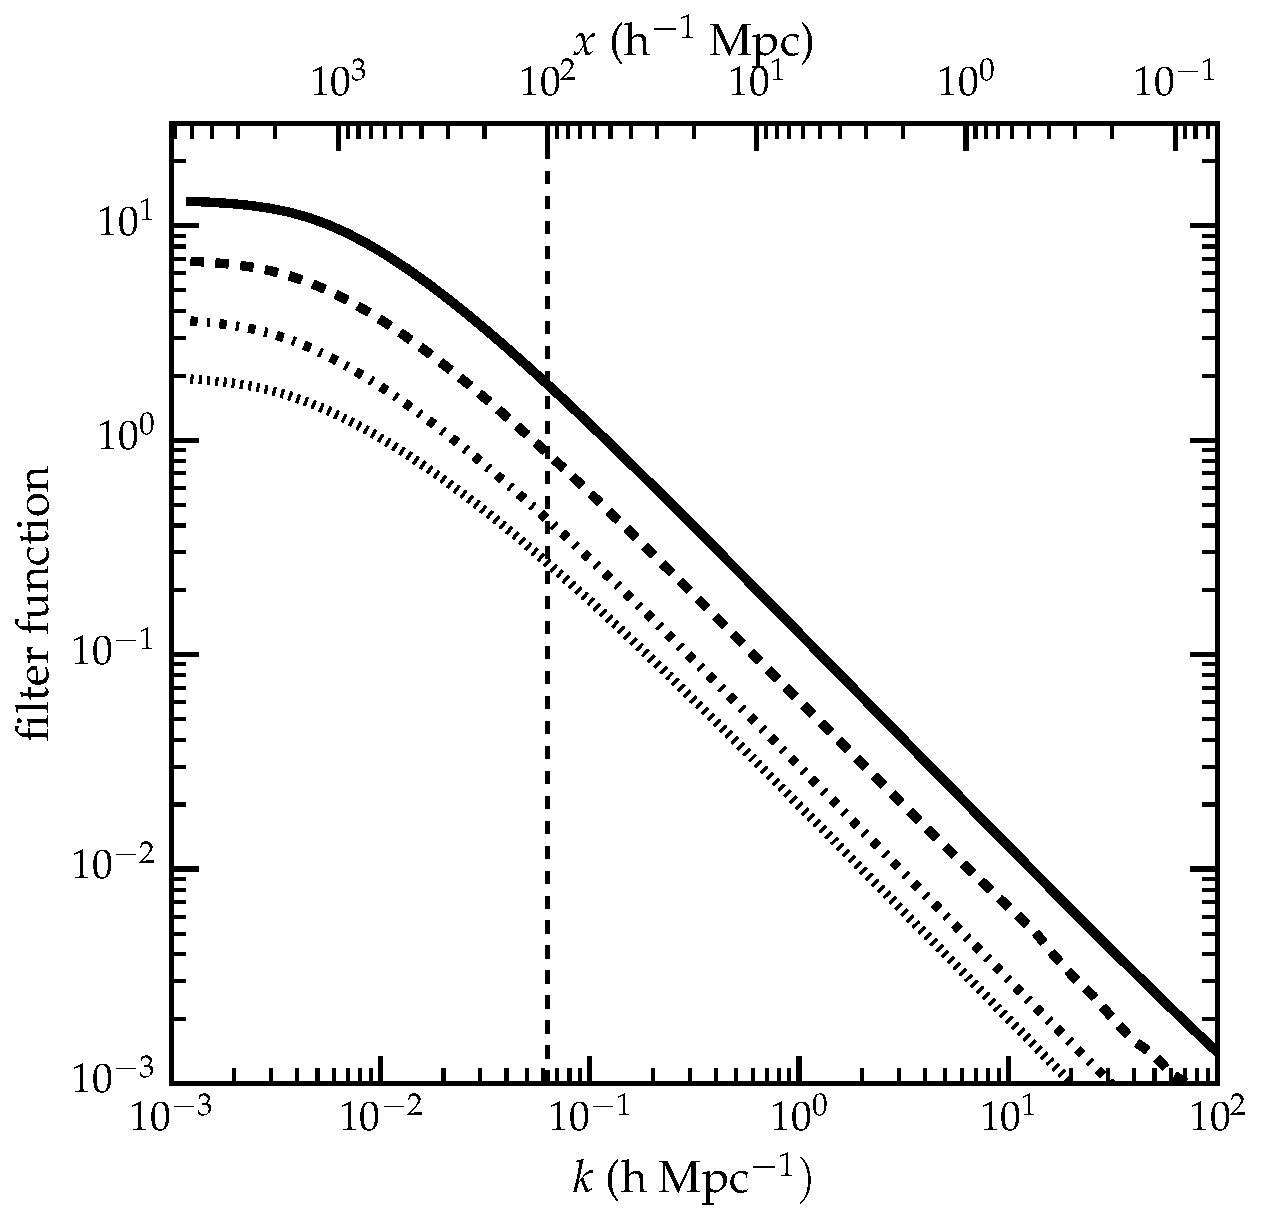
\includegraphics[width = .45\textwidth ]{window_qso}
\caption{Window function for TeV blazar heating for $z=1$ (dotted line), $z=2$ (dot-dashed line), $z=3$ (dashed line)  and $z=4$ (solid line).  The vertical dashed line indicate the minimal comoving wavenumber modeled in the simulation.}
\label{fig:window}
\end{figure}

Because of the typical length scale of the heating rate fluctuations, our simulation have a comoving sidelength of  a $100$ h$^{-1}$ Mpc.  Tests in Paper I showed that this is a sufficiently large size to properly sample the full range of temperature fluctuations. \ALc{Discuss resolution here}



%We use $N= 2\times 512^3$ particles, which gives a mass of $m_\mathrm{gas}=3.8\times10^{6} h^{-1} M_{\odot}$ and $m_\mathrm{DM}=1.8\times 10^{7} h^{-1} M_{\odot}$ for baryonic and dark matter particles, respectively. We used a comoving gravitational softening length of 7.8 $h^{-1}$ kpc. We checked that the resolution has a barely discernible impact on the results of our simulations by performing test simulations with a comoving side length of 50 $h^{-1}$ Mpc at different resolutions, up to $2\times 512^3$. The spread of the temperature in the low density regions increases with increasing resolution. However, this effect is approaching saturation at a resolution of $N=2\times 256^3$. We find less than $4\%$ difference in the median temperature and less than $10\%$ difference in its root mean square in low density regions between $N=2\times 256^3$ and $2\times 512^3$ simulations, indicating that our chosen resolution is sufficient to accurately capture the temperature-density distribution. 

% Photoheating is set by ionization equilibrium of H, He\,\textsc{I} and He\,\textsc{II} in the presence of an external UV field, which is parameterized according to \citet{2009ApJ...703.1416F}. As our version of the \textsc{GADGET-3} code assumes ionization equilibrium when computing photoheating rates, the heating is rather inefficient during reionization where this assumption is not well satisfied \citep[see e.g.][]{2014arXiv1410.1531P}. Following \citet{2012MNRAS.423..149P} we thus include the equivalent heat input by hand at redshift $z=10$. Our simulation does not include radiative transfer effects on the photoionization of He\,\textsc{II}.



\section{Comparison with observations}\label{sec:obs}
\subsection{Inhomegenous blazar heating}
Fig.~\ref{fig:rho_T} shows the temperature-density distribution in our inhomogeneous heating model. The complete description of the inhomogeneous heating model are described in Paper I. Here we recall the main characteristics of the temperature-density distribution, which most observations try to infer. As time goes by, the cumulated impact of blazar heating increases, with a higher temperature difference with respect to the unheated case. Still, as some regions are too far from heating sources, they remain cold, as can be seen by the remnant cold gas, especially at $z=3$. This is very different from the uniform heating model (shown in black) and can potentially reconcile the blazar heating model with observations of absorption lines with Doppler parameter ($b\leq 20$ km s$^{-1}$). At the redshifts most accessible with the Ly$\alpha$ forest, the temperature range  covers almost two orders of magnitude at the lowest density and  even around mean density, there is an important spread. At lower redshifts, the whole IGM gets heated up and after $z\geqslant1$, the inhomogeneous model recovers the uniform model.  In the following section, we compare the observables derived from this $T-\rho$ distribution with observational data.



\begin{figure*}
\centering
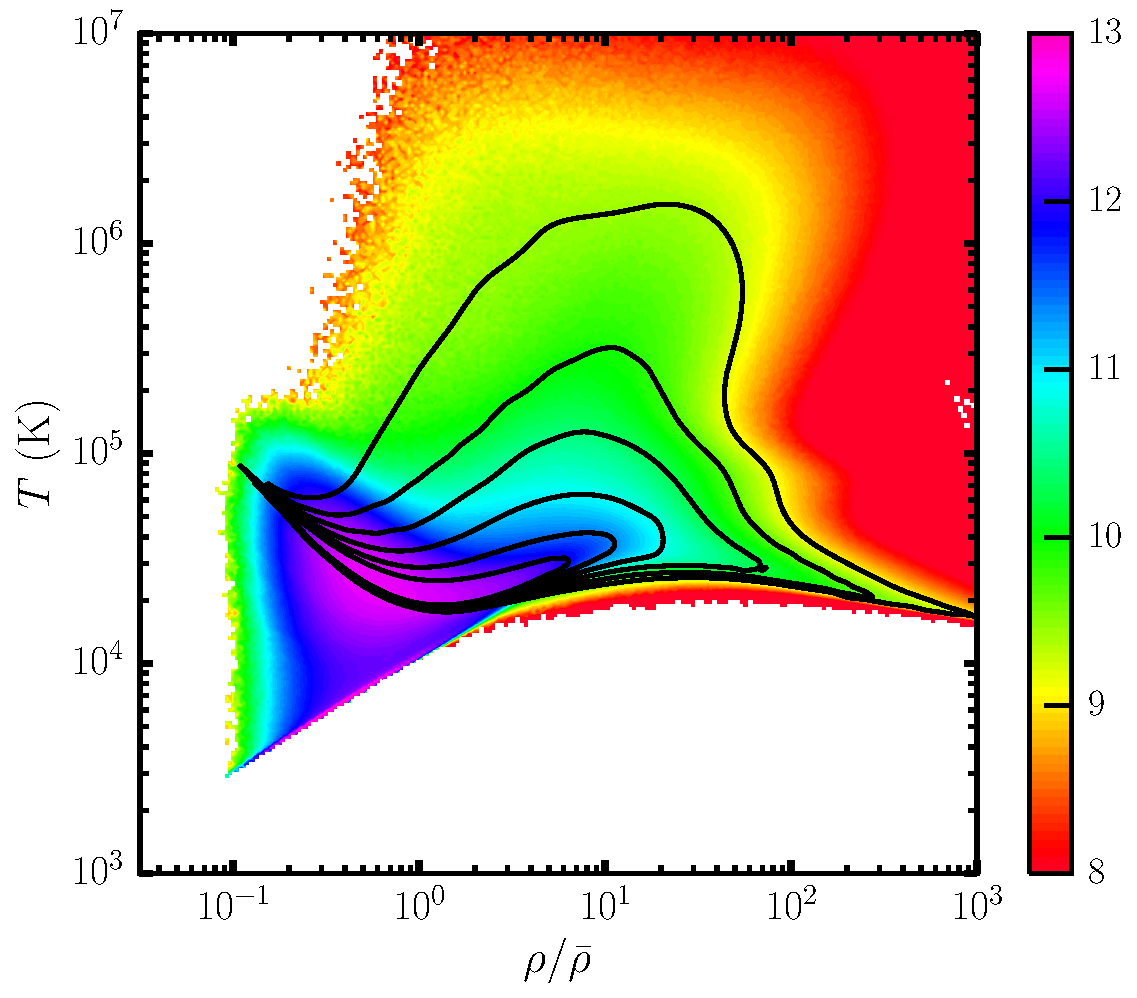
\includegraphics[width = .3\textwidth ]{T_rho_z3_qso.pdf}
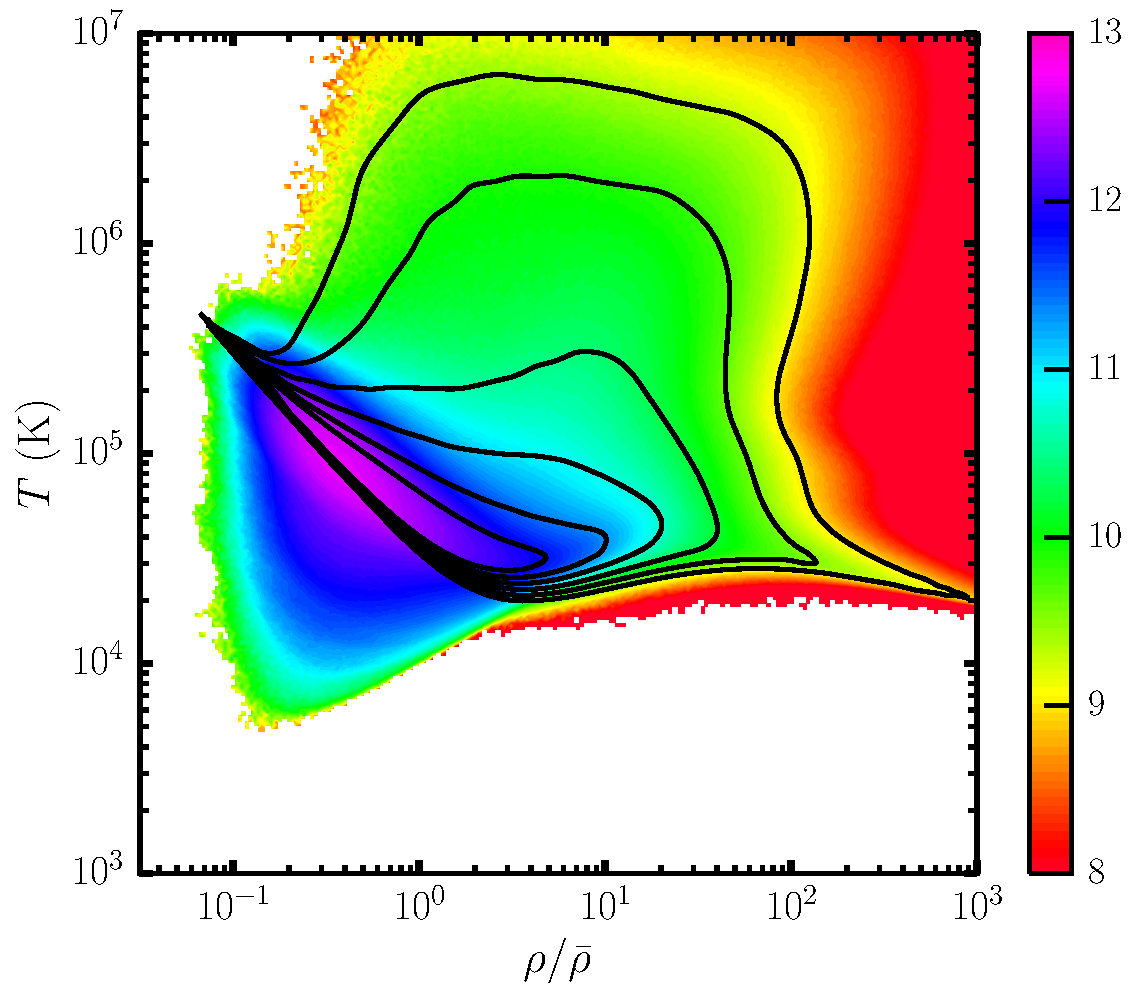
\includegraphics[width = .3\textwidth ]{T_rho_z2_qso.pdf}
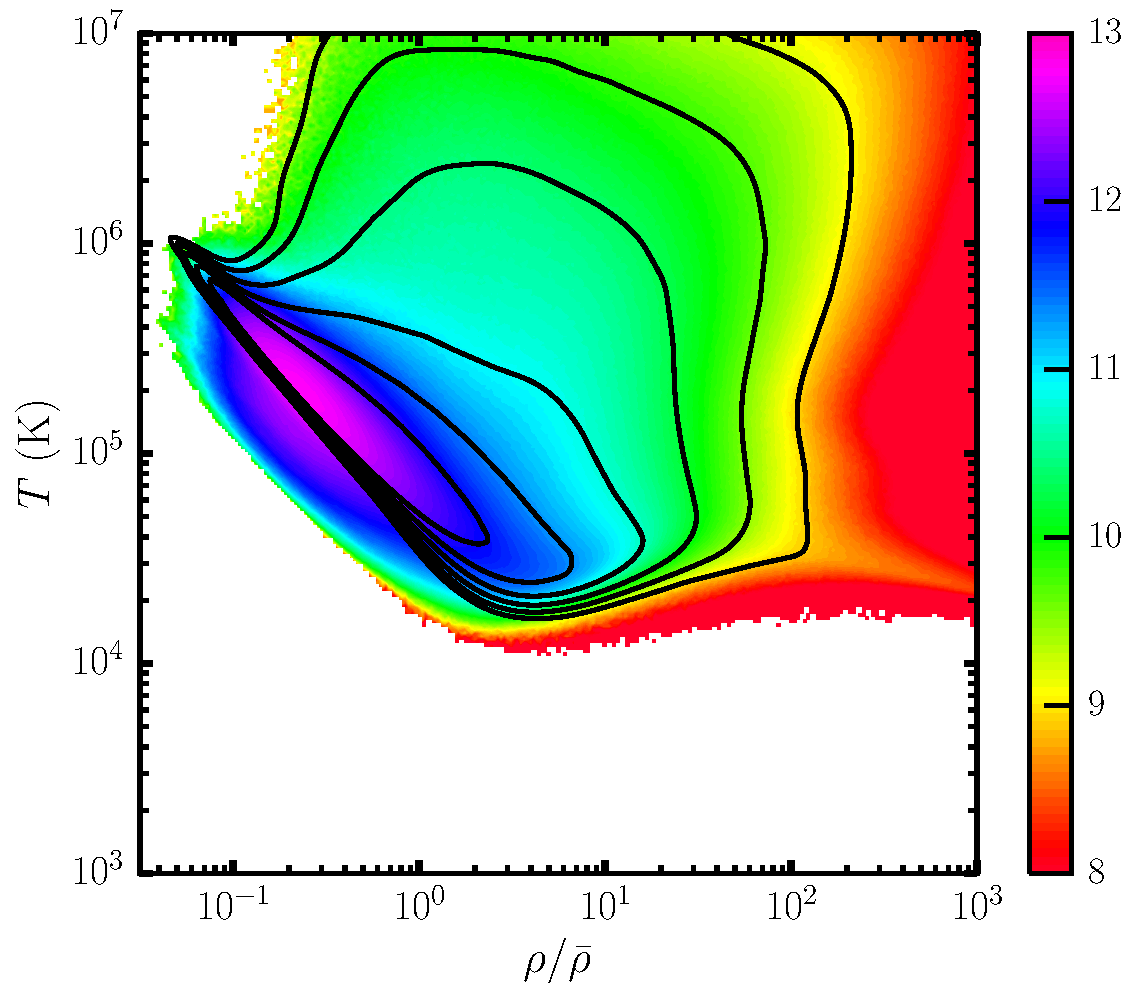
\includegraphics[width = .3\textwidth ]{T_rho_z1_qso.pdf}
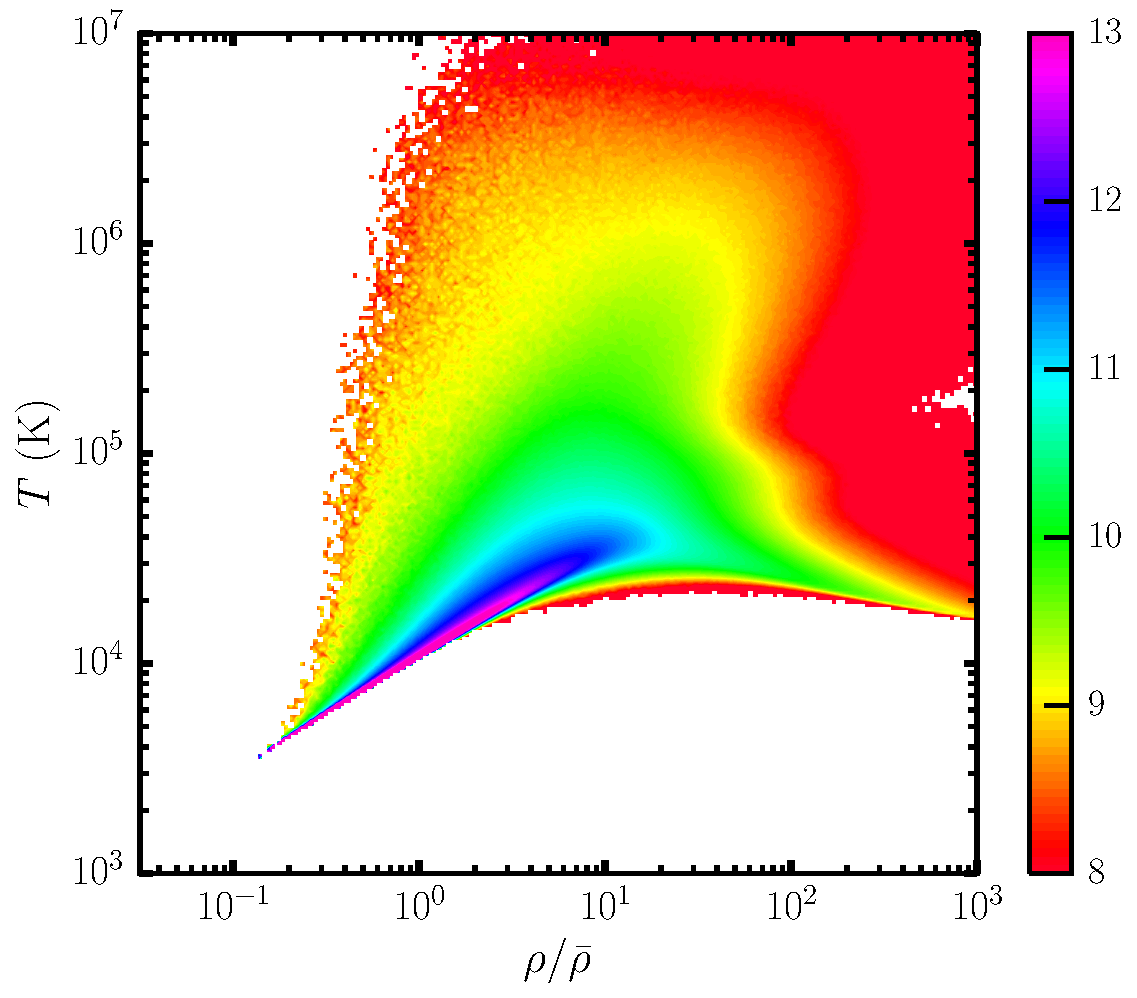
\includegraphics[width = .3 \textwidth ]{T_rho_z3_noheat.pdf}
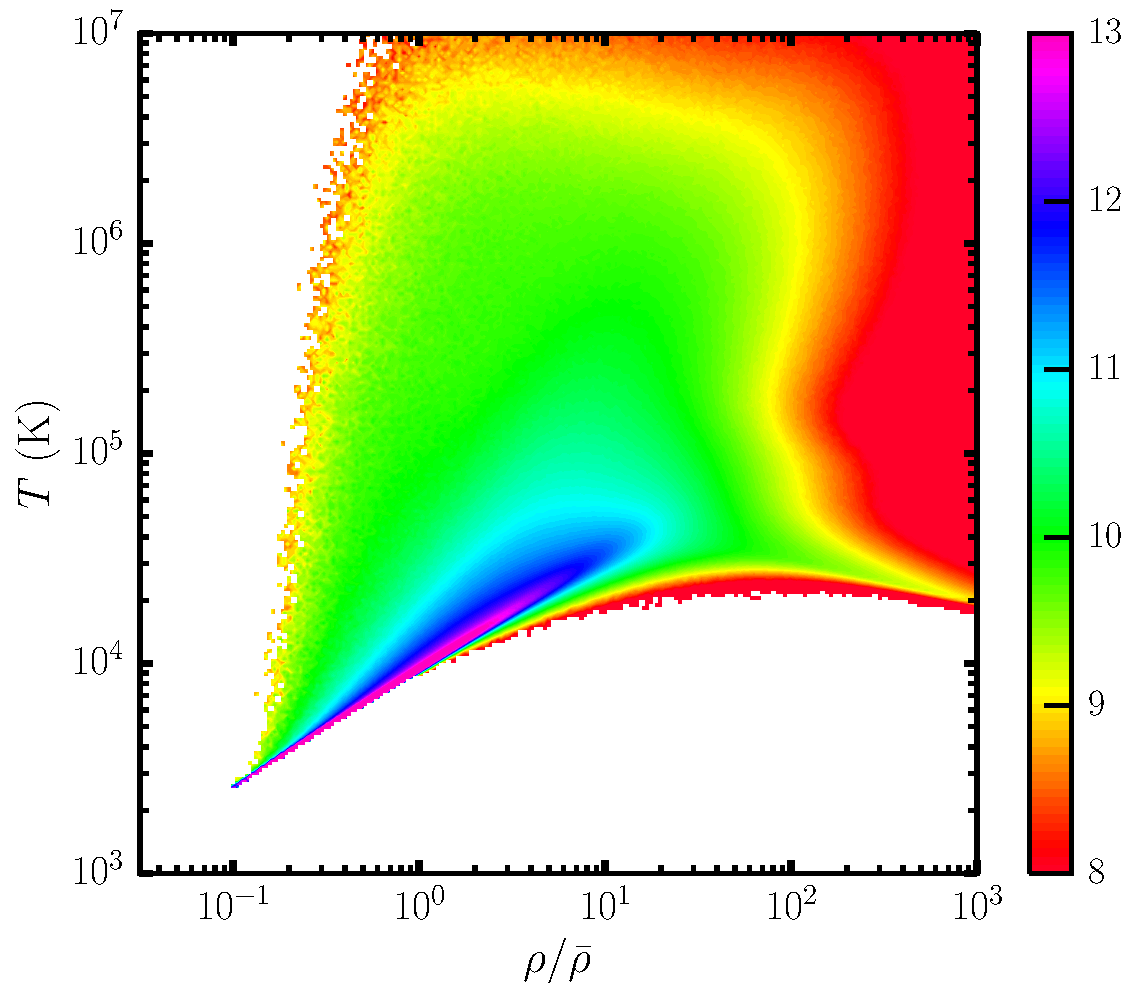
\includegraphics[width = .3\textwidth ]{T_rho_z2_noheat.pdf}
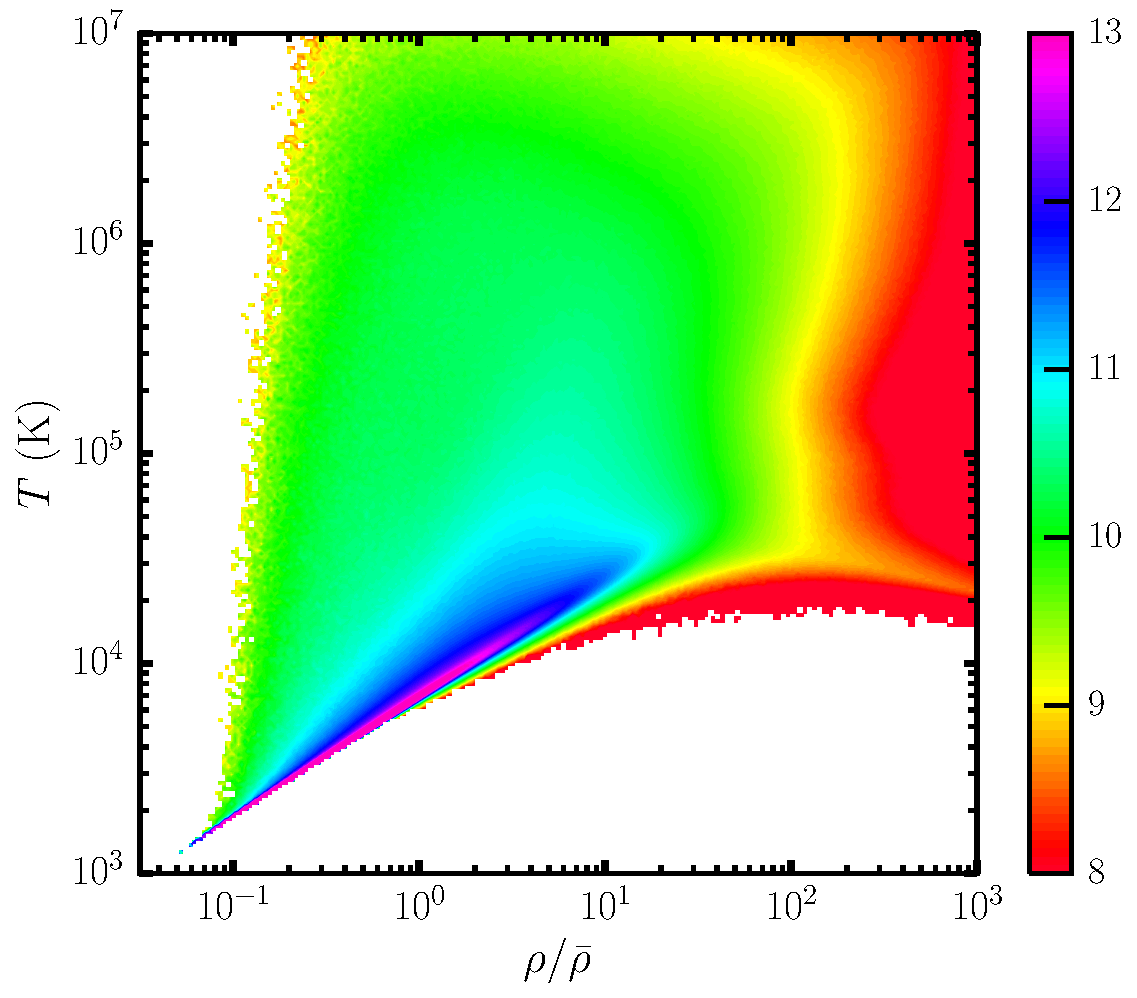
\includegraphics[width = .3\textwidth ]{T_rho_z1_noheat.pdf}

\caption{ Volume-weighted temperature - density relation at $z=3,2$ and 1 (from right to left) for the simulations with no blazar heating (bottom) and inhomogeneous heating (top). The overlying black contours show the corresponding $T-\rho$ relation for uniform blazar heating \citep{2012MNRAS.423..149P} for the same redshift range. The color scale is logarithmic.}

%% 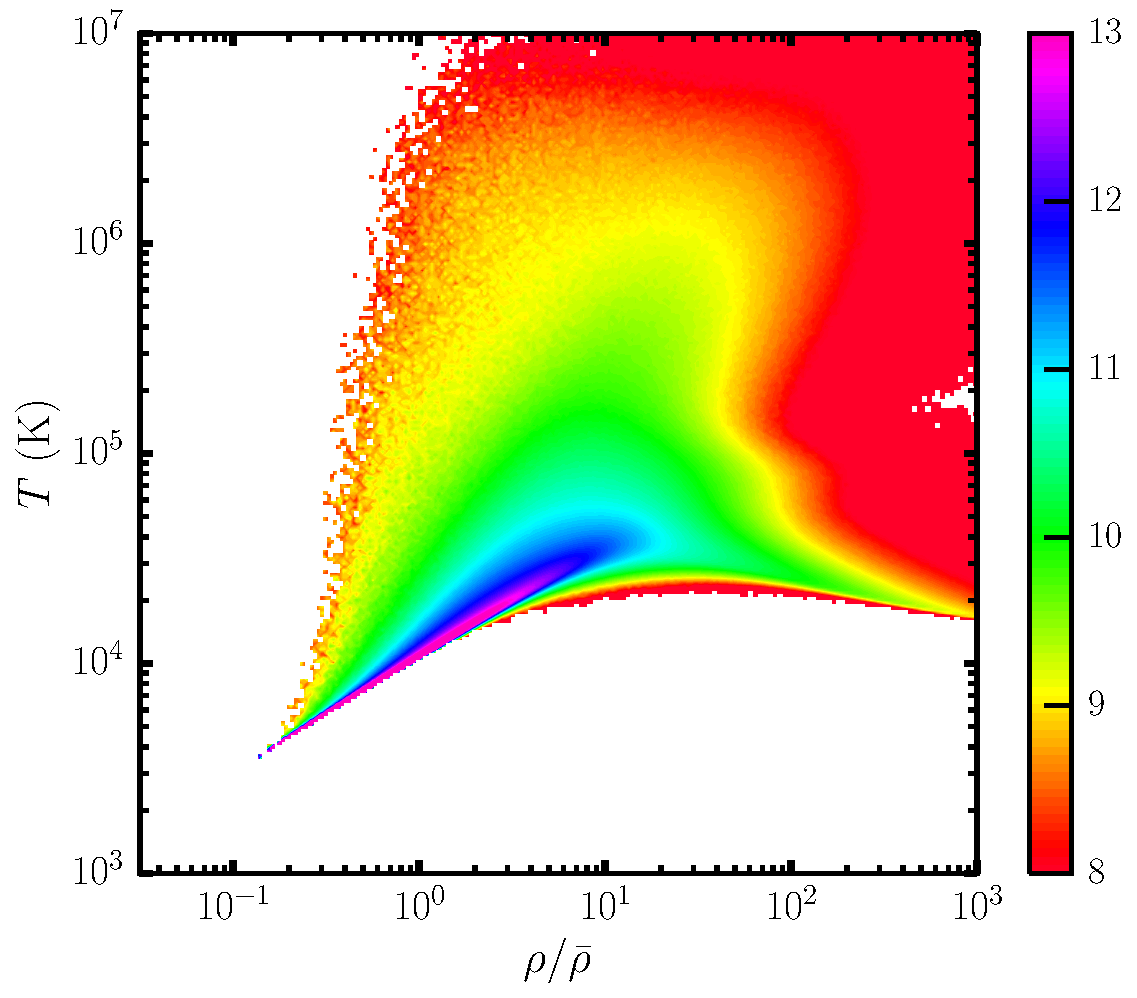
\includegraphics[width = .45\textwidth ]{T_rho_z3_noheat.pdf}
%% 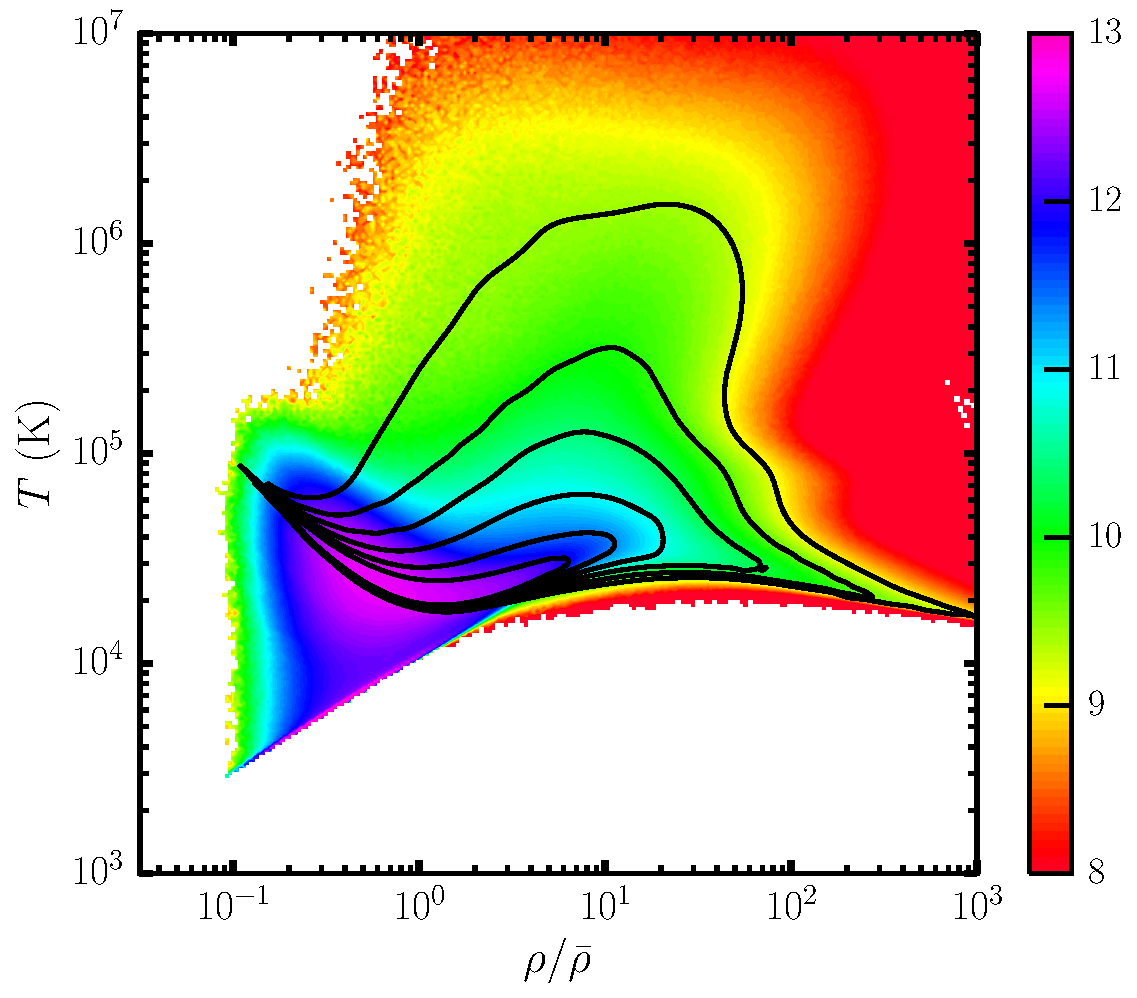
\includegraphics[width = .45\textwidth ]{T_rho_z3_qso.pdf}\\
%% 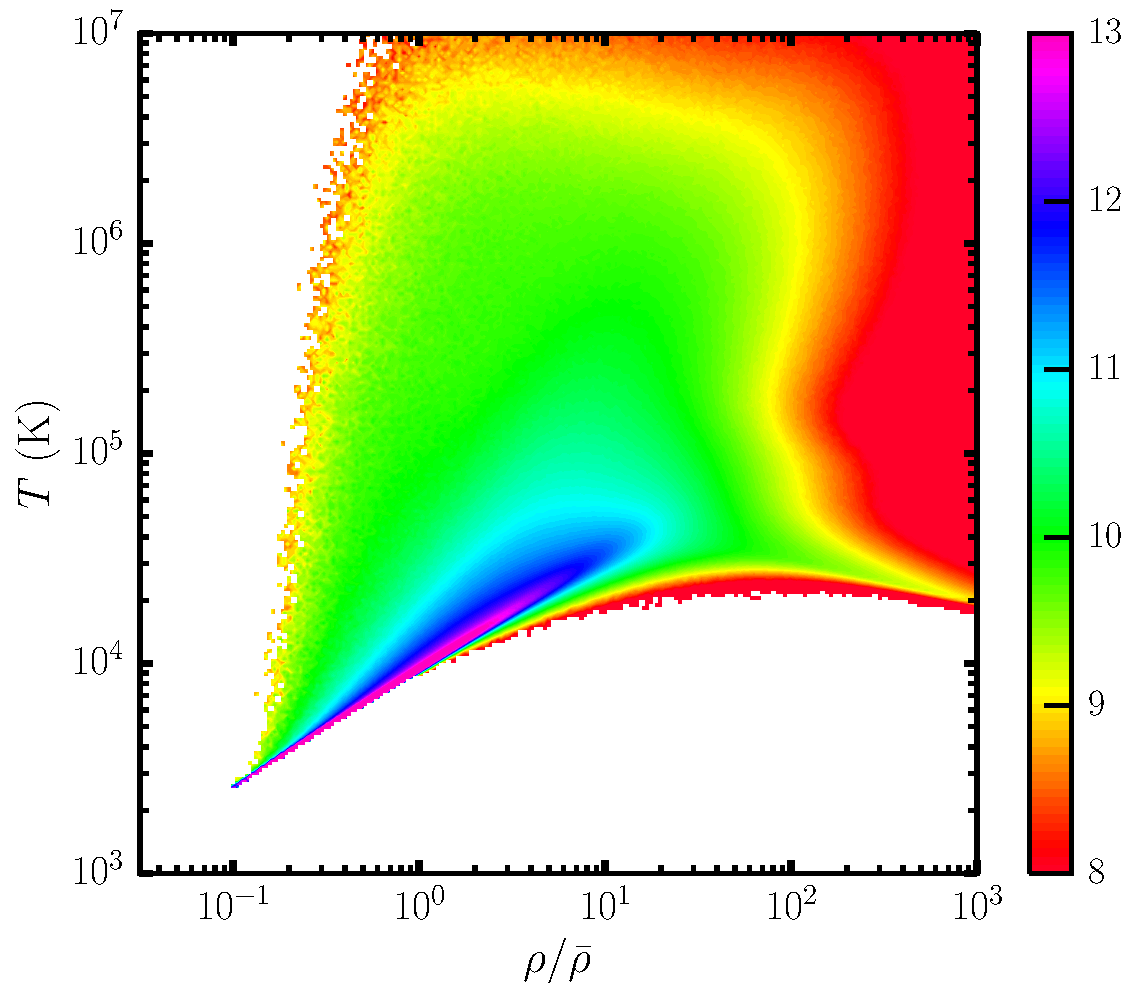
\includegraphics[width = .45\textwidth ]{T_rho_z2_noheat.pdf}
%% 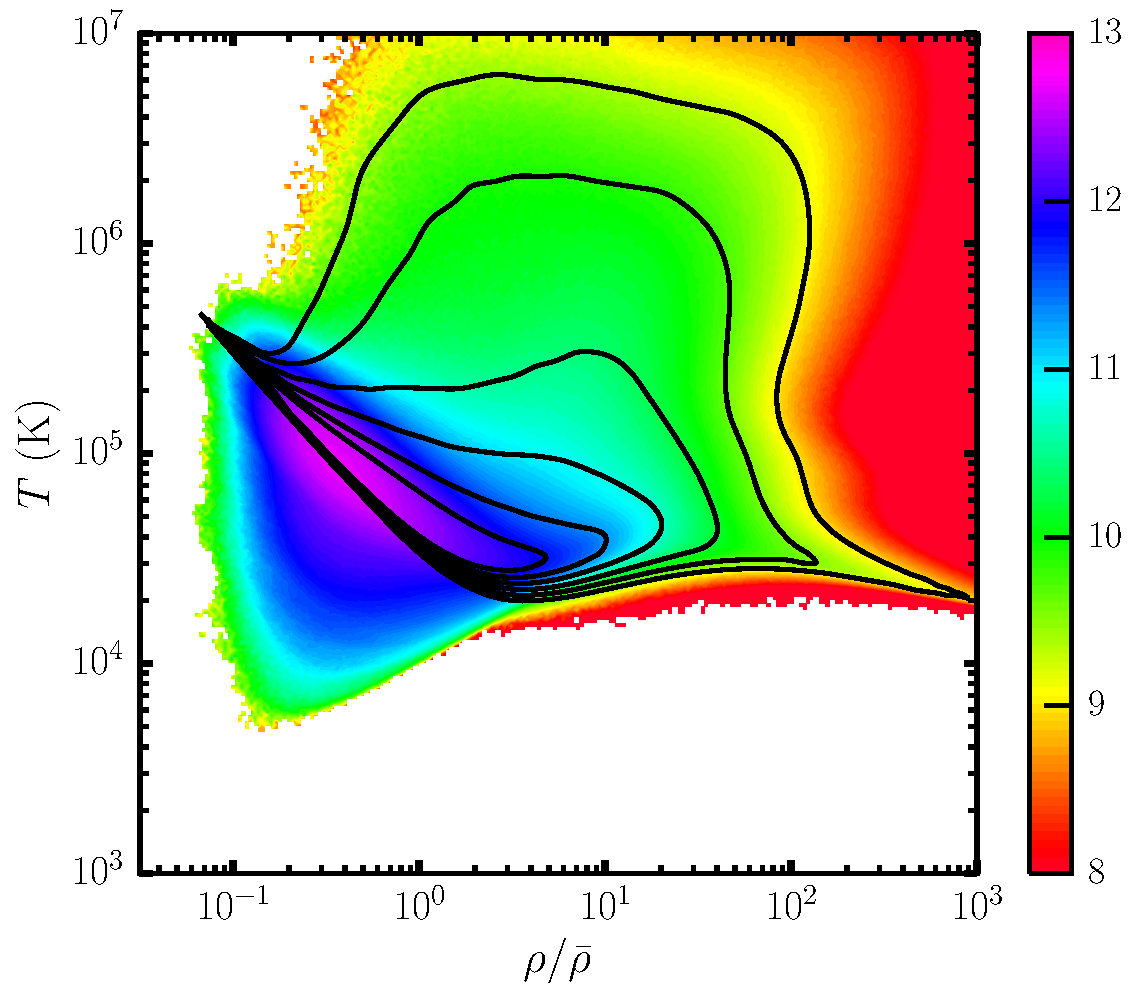
\includegraphics[width = .45\textwidth ]{T_rho_z2_qso.pdf}\\
%% 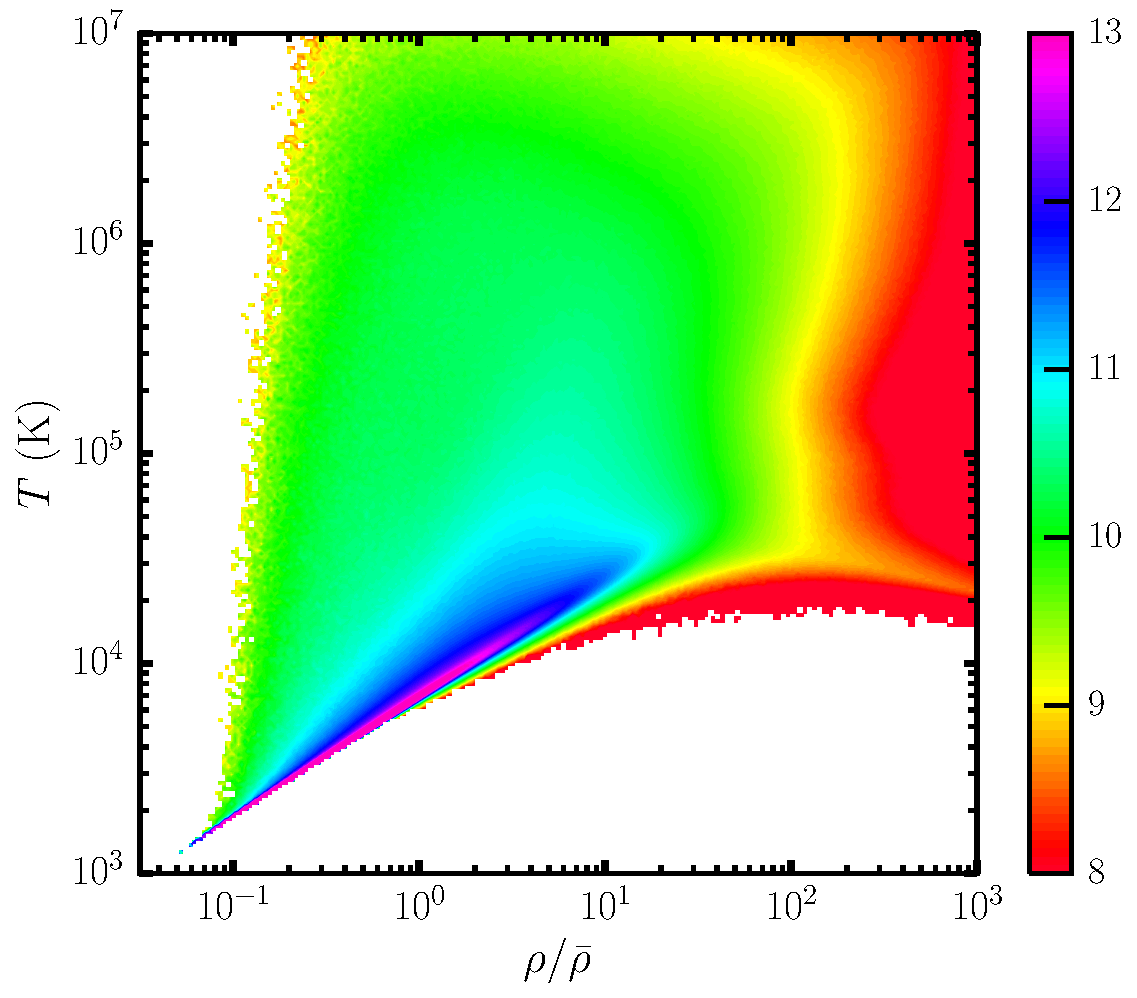
\includegraphics[width = .45\textwidth ]{T_rho_z1_noheat.pdf}
%% 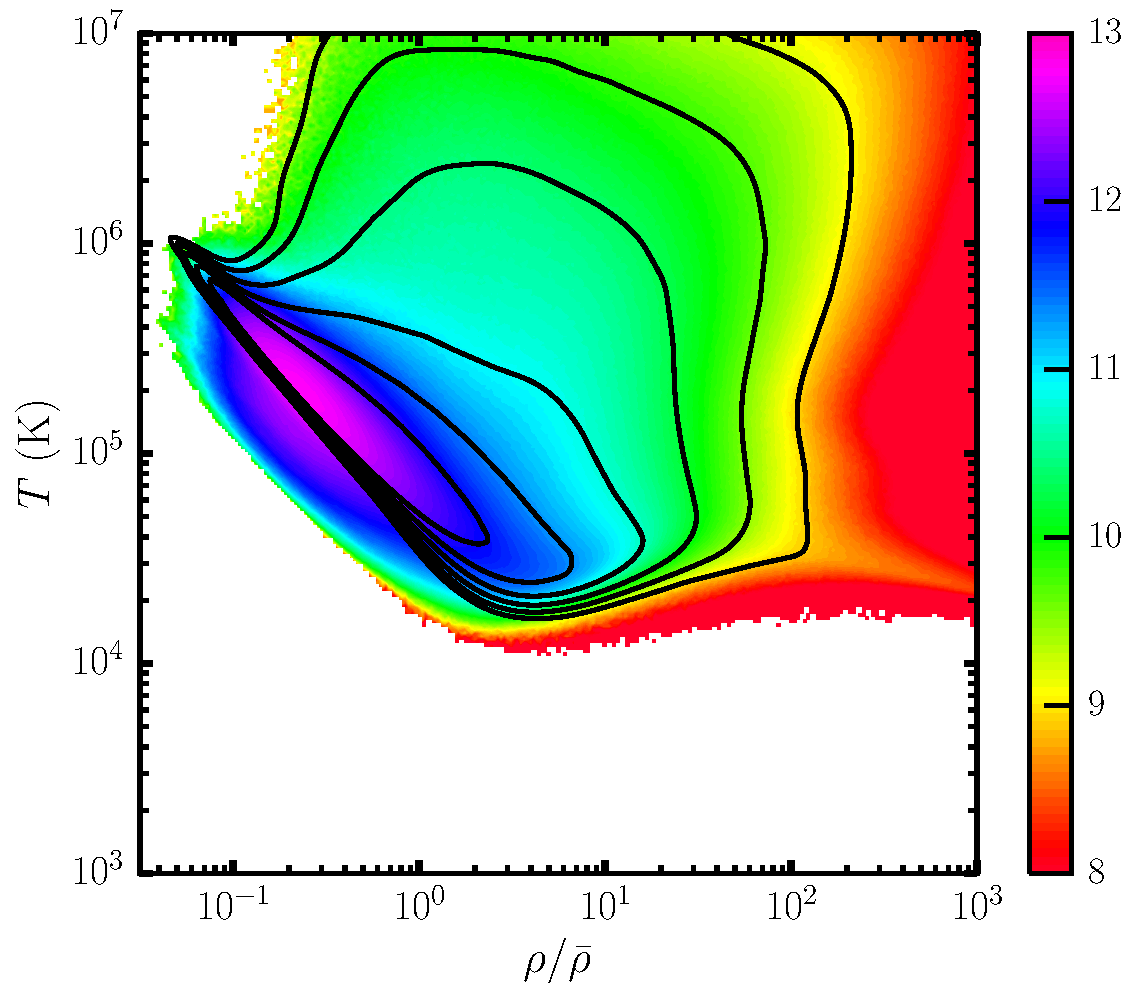
\includegraphics[width = .45\textwidth ]{T_rho_z1_qso.pdf}\\
%% \caption{ Volume-weighted temperature - density relation at $z=3$ (top), $z=2$ (middle), $z=1$ (bottom) for the simulations with no blazar heating (left) and inhomogeneous heating (right). The overlying black contours show the corresponding $T-\rho$ relation for uniform blazar heating \citep{2012MNRAS.423..149P} for the same redshift range. The color scale is logarithmic.}


\label{fig:rho_T}
\end{figure*}




\subsection{Post-processing the simulations}
\begin{itemize}
\item Global flow , potential caveats
\item Details about subdividing LOS in chunks for VPFIT
\end{itemize}

\begin{figure*}[h]
\centering
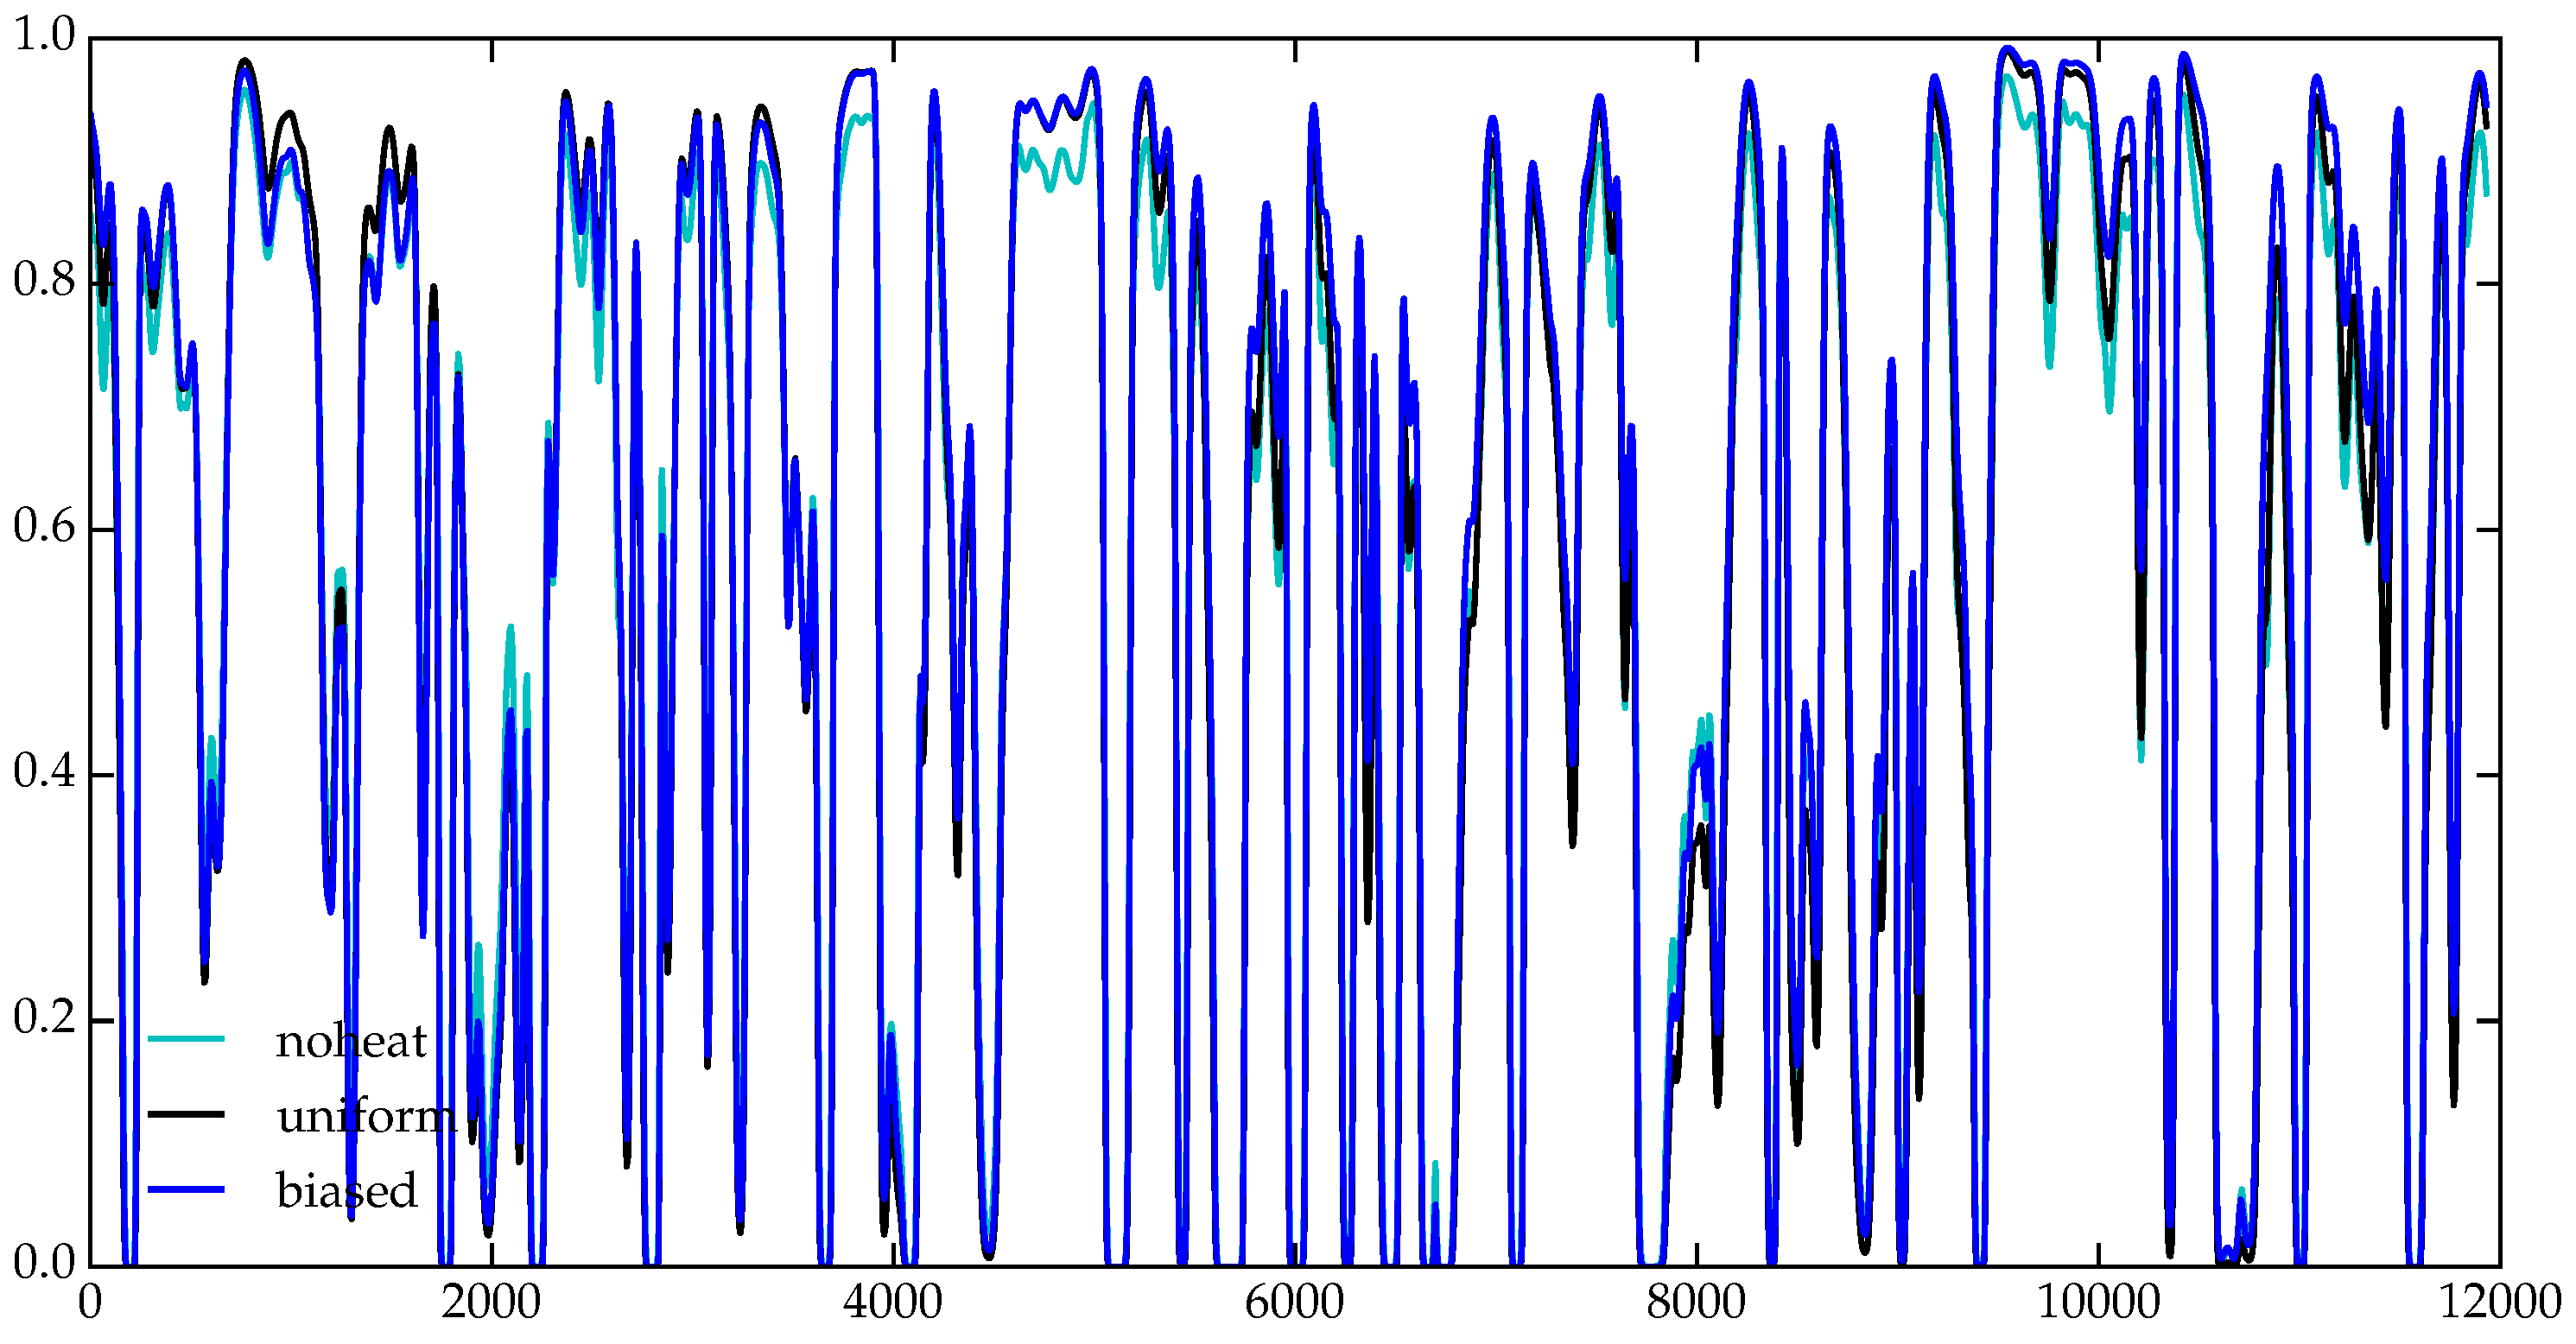
\includegraphics[width = .8\textwidth ]{lines_z2_2}
\caption{Ly$\alpha$ absorption spectrum at $z=2.2$ in the three models. \ALc{[Placeholder, will be improved]}}
\label{fig:bias}
\end{figure*}

\subsection{Ly$\alpha$ forest statistics}


\begin{figure}[h]
\centering
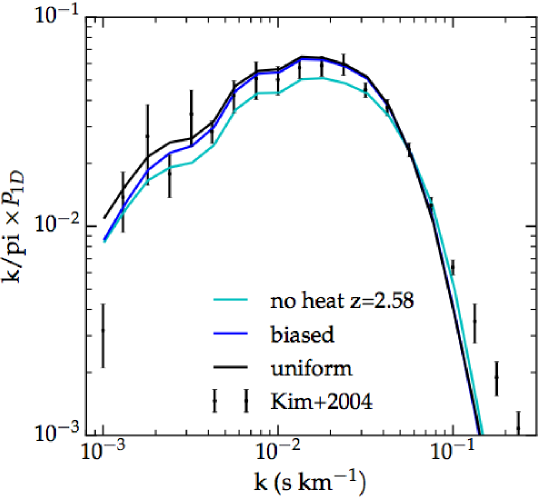
\includegraphics[width = .45\textwidth ]{powerspec}
\caption{ Power spectrum at different redshifts compare with observations \ALc{[Placeholder, will be improved]}}
\label{fig:powespec}
\end{figure}

\begin{figure*}[h]
\centering
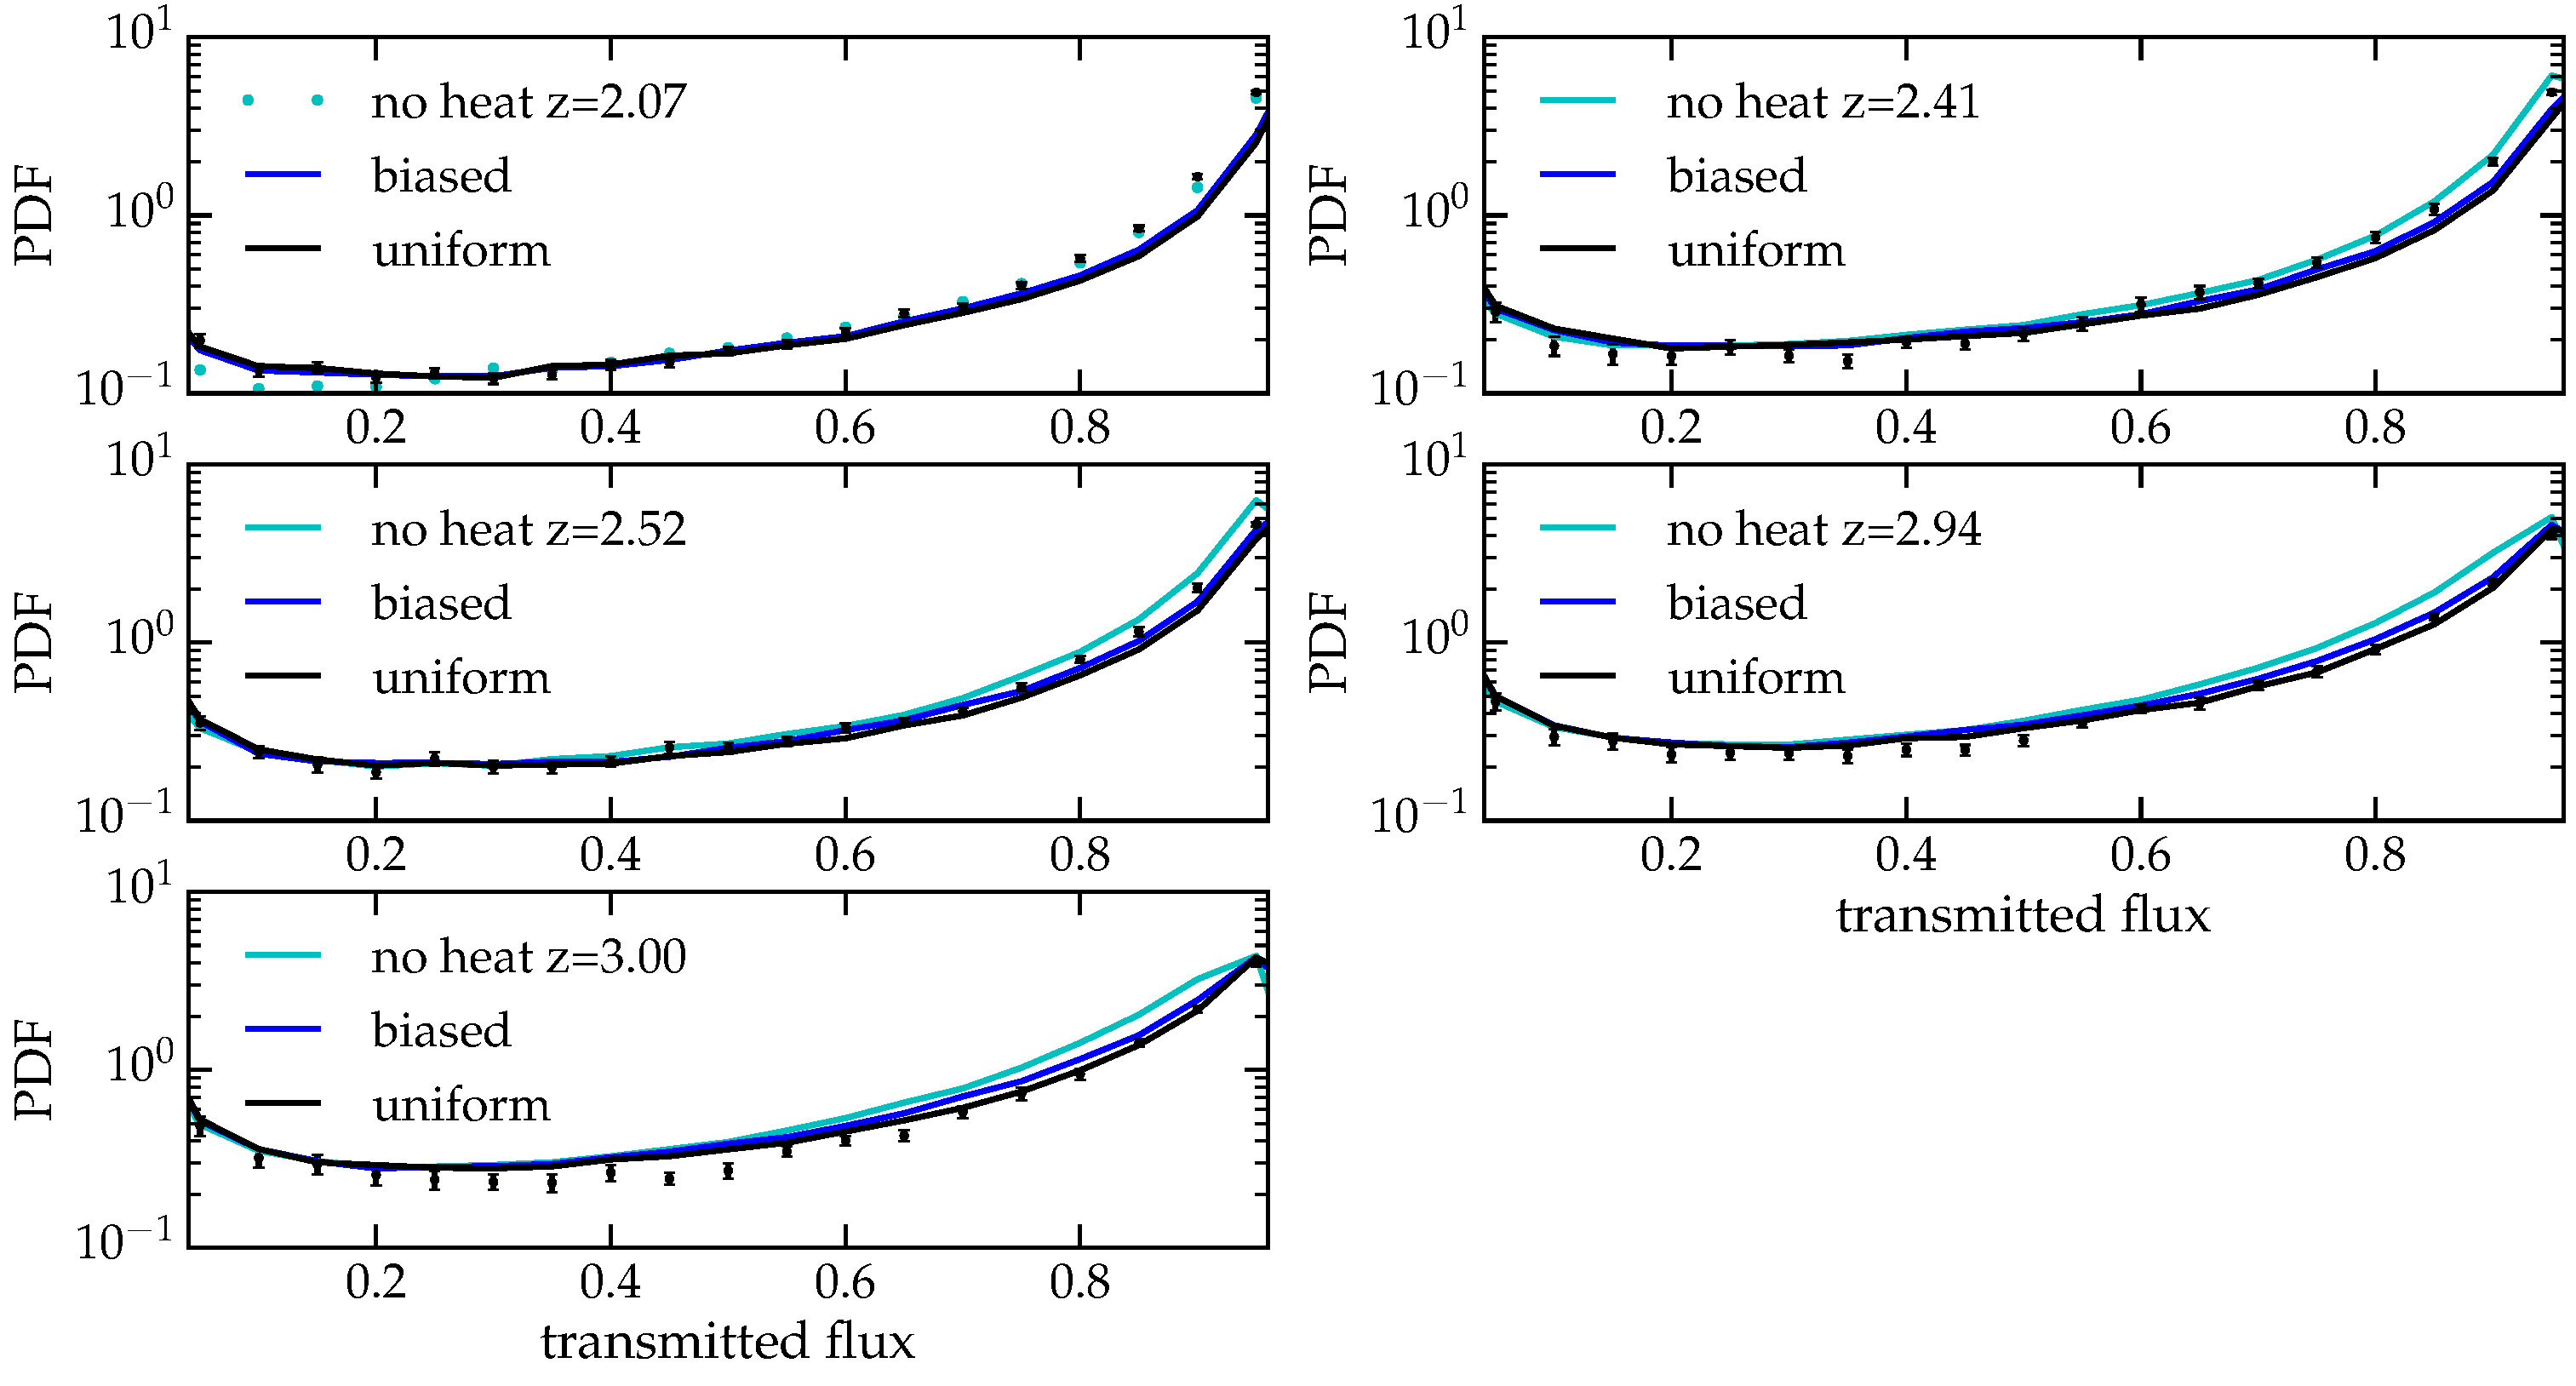
\includegraphics[width = .9\textwidth ]{flux_PDF}
\caption{Flux PDF at different redshifts compare with observations \ALc{[Placeholder, will be improved]}}
\label{fig:fluxPDF}
\end{figure*}

\subsection{Thermal state of the IGM}
\begin{enumerate}
\item Compare with Rorai 2016
\item Maybe compare with low-z results
\item Rudie and other b-Nh distributions
\end{enumerate}
\begin{figure}
\centering
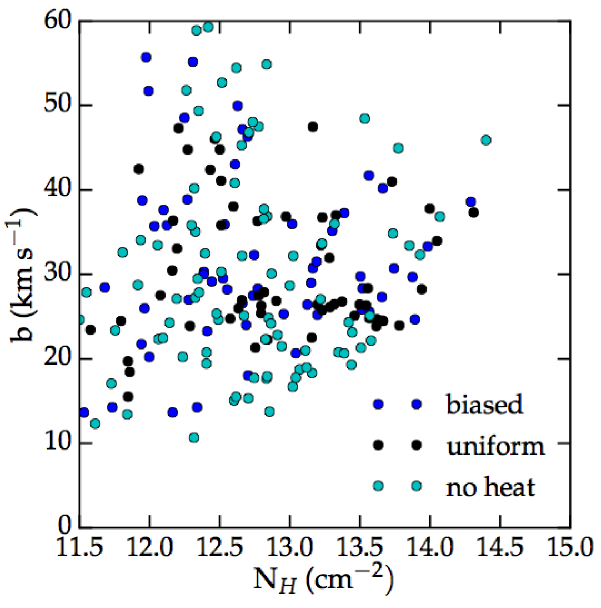
\includegraphics[width = .45\textwidth ]{b_Nh}
\caption{ Column density - Doppler with distribution in the different models \ALc{[Placeholder, will be improved]}}
\label{fig:b_Nh}
\end{figure}



\section{Discussion}\label{sec:discussion}

\section{Conclusions}\label{sec:conclusion}

\begin{acknowledgements}
%% AL and PC are supported by the UWM Research Growth Initiative, the NASA ATP
%% program through NASA grant NNX13AH43G, and NSF grant AST-1255469.
%% A.E.B.~and M.S.~receive financial support from the Perimeter
%% Institute for Theoretical Physics and the Natural Sciences and
%% Engineering Research Council of Canada through a Discovery Grant.
%% Research at Perimeter Institute is supported by the Government of
%% Canada through Industry Canada and by the Province of Ontario through
%% the Ministry of Research and Innovation.
%% C.P.~gratefully acknowledges
%% financial support of the Klaus Tschira Foundation. E.P. acknowledges support by the ERC grant ``The Emergence of Structure during the epoch of Reionization''.
%% The authors acknowledge the Texas Advanced Computing Center (TACC) at The University of Texas at Austin and the NASA Advanced Supercomputing Division for providing HPC resources that have contributed to the research results reported within this paper. The authors thank S. Furlanetto, A. Loeb and M. Heahnelt for fruitful discussions. 
\end{acknowledgements}

\bibliographystyle{apj}
\bibliography{biblio_total}
\end{document}
